\documentclass[11pt]{article}
% Clean TMLR-like single-column layout. Swap in tmlr.sty for submission.
\usepackage[letterpaper,margin=1in]{geometry}
\usepackage{graphicx}
\usepackage{booktabs}
\usepackage{amsmath}
\usepackage{xcolor}
\usepackage{caption}
\usepackage[colorlinks=true,linkcolor=blue,citecolor=blue,urlcolor=blue]{hyperref}
\captionsetup{font=small,labelfont=bf}
\definecolor{collapse}{HTML}{d1495b}
\newcommand{\collapse}[1]{\textcolor{collapse}{\textbf{#1}}}

\title{\textbf{One Codebook for Every Architecture:\\ Asymmetric NormalFloat for Calibration-Free KV-Cache Quantization}}
\author{Andrew H. Bond}
\date{\today}

\begin{document}
\maketitle

\begin{abstract}
Quantizing the key--value (KV) cache is the standard route to long-context LLM inference,
and the data-free NormalFloat-4 (NF4) codebook is a popular calibration-free choice. We show
that \textbf{NF4 silently and catastrophically fails on an entire class of models}---those
with high-ratio grouped-query attention (GQA)---while appearing excellent on the Llama-family
multi-head-attention (MHA) models that dominate published benchmarks. On Qwen2.5-7B (7:1 GQA),
4-bit NF4 KV-cache quantization collapses LongBench-qasper from \textbf{43.8 (fp16) to 4.7} and
WikiText-2 perplexity from \textbf{7.46 to 74.7}---degenerate repetition---whereas the same
recipe is near-lossless on Llama-2-7B/13B and Mistral-7B. We trace the failure to NF4's
\emph{zero-centred, abs-max} scaling: KV keys carry a large per-channel DC offset, so a
symmetric codebook wastes half of its codes on the empty side, and high-GQA models---which
route each KV-head error into many query heads---cannot absorb the resulting error. The fix is
a single per-channel zero-point: \textbf{asymmetric NF4 (asym-NF4)} centres the codebook on the
data before applying the NF grid. asym-NF4 is one calibration-free codebook that is near-fp16
on \emph{every} architecture we test---it ties symmetric NF4 where NF4 already works and
recovers the Qwen collapse to \textbf{41.9 qasper / 7.50 ppl}---at no extra bit cost. We release
the method, a reproducible cross-model harness, and a practitioner's decision guide.
\end{abstract}

\section{Introduction}
The KV cache dominates the memory footprint of long-context inference, and 4-bit quantization
of keys and values is now standard practice. Calibration-free codebooks are attractive because
they require no data pass: the 4-bit NormalFloat (NF4) grid, popularised by QLoRA, allocates
levels by a unit Gaussian and is a common default for KV keys. Most KV-quantization studies
benchmark on the Llama family. We show that this hides a \emph{silent, catastrophic} failure.

\paragraph{Contributions.}
\begin{enumerate}
  \item A silent, catastrophic failure mode of NF4 KV quantization on high-GQA models
        (Qwen2.5), invisible on the Llama-family models typically benchmarked
        (Fig.~\ref{fig:crossover}, Fig.~\ref{fig:ppl}).
  \item A measured mechanism: NF4 costs ${\sim}4\times$ the per-channel reconstruction error of
        asymmetric uniform on DC-offset KV keys, and high-GQA error amplification turns that
        error into collapse. Bit-depth is \emph{not} the axis---3-bit \emph{uniform} beats
        4-bit NF4 on Qwen (Fig.~\ref{fig:rescue}, Fig.~\ref{fig:mechanism}).
  \item \textbf{asym-NF4}: a one-line per-channel zero-point that unifies the codebook
        choice---best-or-tied on every architecture, calibration-free, no extra bits
        (Fig.~\ref{fig:asymnf4}).
  \item A reproducible single harness, a cross-model matrix, and a practitioner decision guide.
\end{enumerate}

\section{Background and setup}
We quantize keys per channel and values per token, with optional dense-and-sparse fp16
outliers (top 2\% magnitude per channel) and an attention sink, in a deployable prefill-once
cache that runs at ${\sim}$fp16 speed. We compare four calibration-free key codebooks at 4 bits:
fp16 (reference), symmetric NF4 (abs-max scaling about zero), asymmetric uniform (per-group
min/max), and our asym-NF4. Models span the GQA spectrum: Llama-2-7B/13B (MHA, 1:1), Mistral-7B
(GQA 4:1), Qwen2.5-7B (GQA 7:1). We evaluate on the LongBench English subset and WikiText-2
perplexity. All scores are produced by a single harness and are only compared intra-harness.

\section{NF4 fails on high-GQA models}
\label{sec:headline}
Figure~\ref{fig:crossover} and Table~\ref{tab:qasper} give the headline. NF4 is the best naive
codebook on Llama-2-7B/13B and Mistral, but on Qwen2.5-7B it \collapse{collapses} from 43.8
(fp16) to 4.7---near-random, degenerate repetition. Asymmetric uniform never collapses but
sacrifices 5--9 qasper points on the MHA models. asym-NF4 is best-or-tied everywhere.
Perplexity tells the identical story (Fig.~\ref{fig:ppl}, Table~\ref{tab:ppl}): on Qwen,
symmetric NF4 perplexity explodes $10\times$ (7.46$\rightarrow$74.2) while asym-NF4 holds at 7.50.

\begin{figure}[t]
\centering
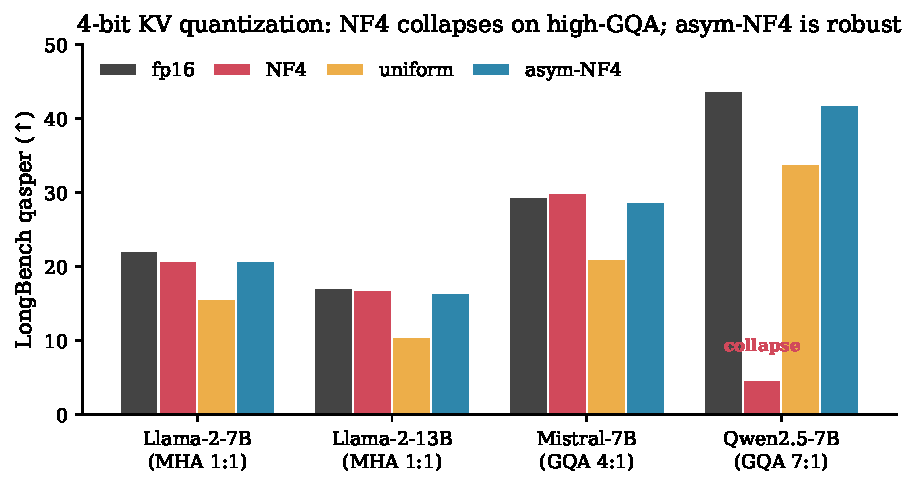
\includegraphics[width=\linewidth]{fig_crossover.pdf}
\caption{4-bit KV quantization on the LongBench qasper task. NF4 (red) is competitive on the
MHA / low-GQA models but \collapse{collapses} on Qwen2.5-7B (7:1 GQA). asym-NF4 (blue) is
near-fp16 on every architecture.}
\label{fig:crossover}
\end{figure}

\begin{table}[t]
\centering\small
\caption{LongBench qasper ($\uparrow$), 4-bit keys, identical outliers/sink.}
\label{tab:qasper}
\begin{tabular}{llrrrr}
\toprule
model & attn (Q:KV) & fp16 & NF4 & uniform & \textbf{asym-NF4} \\
\midrule
Llama-2-7B  & MHA 1:1 & 22.06 & 20.82 & 15.58 & \textbf{20.81} \\
Llama-2-13B & MHA 1:1 & 17.06 & 16.86 & 10.52 & \textbf{16.41} \\
Mistral-7B  & GQA 4:1 & 29.43 & 29.96 & 21.06 & \textbf{28.74} \\
Qwen2.5-7B  & GQA 7:1 & 43.77 & \collapse{4.69} & 33.81 & \textbf{41.91} \\
\bottomrule
\end{tabular}
\end{table}

\begin{figure}[t]
\centering
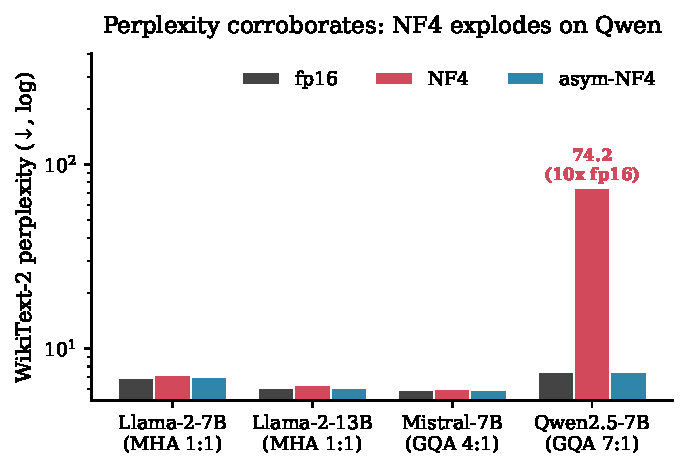
\includegraphics[width=0.72\linewidth]{fig_perplexity.pdf}
\caption{WikiText-2 perplexity ($\downarrow$, log scale). Symmetric NF4 explodes $10\times$ on
Qwen2.5-7B; asym-NF4 sits on fp16 everywhere.}
\label{fig:ppl}
\end{figure}

\begin{table}[t]
\centering\small
\caption{WikiText-2 perplexity ($\downarrow$), same recipe.}
\label{tab:ppl}
\begin{tabular}{lrrr}
\toprule
model & fp16 & NF4 & \textbf{asym-NF4} \\
\midrule
Llama-2-7B  & 6.94 & 7.18 & \textbf{6.97} \\
Llama-2-13B & 6.11 & 6.30 & \textbf{6.13} \\
Mistral-7B  & 5.94 & 6.00 & \textbf{5.96} \\
Qwen2.5-7B  & 7.46 & \collapse{74.19} & \textbf{7.50} \\
\bottomrule
\end{tabular}
\end{table}

\section{Anatomy of the collapse}
\paragraph{It is the codebook shape, not the bit-depth.}
Figure~\ref{fig:rescue} isolates the cause on Qwen. Holding the model fixed, 4-bit NF4 scores
4.7; 4-bit \emph{uniform} scores 33.8; and \emph{3-bit} uniform scores 34.9---lower precision,
$7\times$ better. Adding 10\% fp16 outliers, shortening the context, or raising values to 8-bit
all leave NF4 collapsed. Only changing the codebook helps.

\paragraph{Mechanism.}
On real pre-RoPE keys, NF4 incurs ${\sim}3$--$5\times$ the per-channel relative reconstruction
error of asymmetric uniform---on \emph{both} Qwen and Llama (Fig.~\ref{fig:mechanism})---because
KV keys carry a per-group DC offset (range/abs-max $\approx 0.9$) and NF4's zero-centred grid
spends about half of its codes on the empty side (Fig.~\ref{fig:asymnf4}). Crucially, NF4's key
error is \emph{equal} across the two models, so representation alone does not explain the
collapse. The differentiator is \textbf{error tolerance}: Qwen's 7:1 GQA routes each KV-head
error into seven query heads, whereas Llama-2-7B (1:1 MHA) routes it into one. Qwen collapses
above a key-relerr threshold between 0.04 (uniform-3b) and 0.08 (NF4-4b); Llama's threshold
exceeds 0.08.

\begin{figure}[t]
\centering
\begin{minipage}{0.49\linewidth}\centering
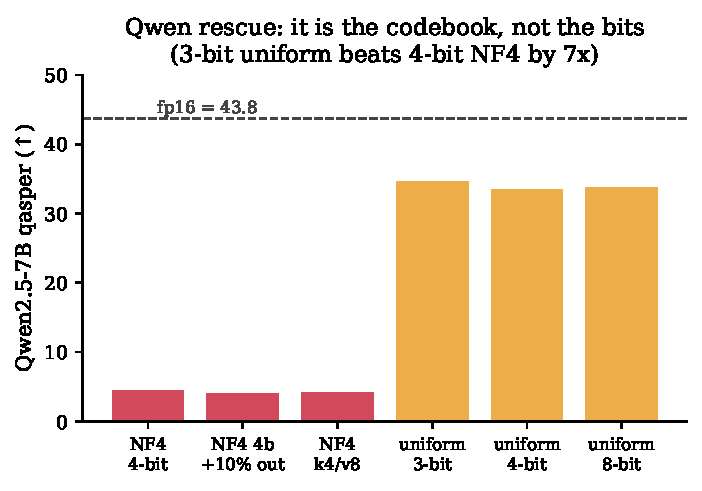
\includegraphics[width=\linewidth]{fig_rescue.pdf}
\caption{Qwen rescue sweep. The codebook---not the bit budget---decides survival.}
\label{fig:rescue}
\end{minipage}\hfill
\begin{minipage}{0.49\linewidth}\centering
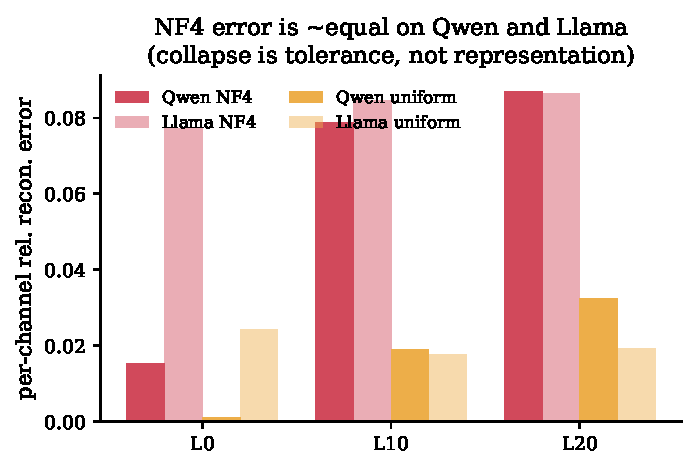
\includegraphics[width=\linewidth]{fig_mechanism.pdf}
\caption{NF4's reconstruction error is ${\sim}$equal on Qwen and Llama; the collapse is error
\emph{tolerance}, not representation.}
\label{fig:mechanism}
\end{minipage}
\end{figure}

\section{Asymmetric NF4}
asym-NF4 adds a per-channel zero-point. For each channel we subtract the mean $\mu$,
NF4-quantize the residual scaled by its abs-max, and add $\mu$ back at decode:
\[
\hat{x} \;=\; \mu \;+\; \mathrm{absmax}(x-\mu)\cdot \mathrm{NF4}\!\left(\frac{x-\mu}{\mathrm{absmax}(x-\mu)}\right).
\]
This stores one extra fp16 scalar per channel ($\mu$) beyond NF4's abs-max---negligible
(4-bit compression ratio 7.9$\times$, identical to NF4). It keeps NF4's nonlinear levels (so it
\emph{beats} uniform) while centring the grid on the data (so it \emph{does not collapse}).
Figure~\ref{fig:asymnf4} shows the intuition. Tables~\ref{tab:qasper}--\ref{tab:ppl} show
asym-NF4 is best-or-tied on every model.

\begin{figure}[t]
\centering
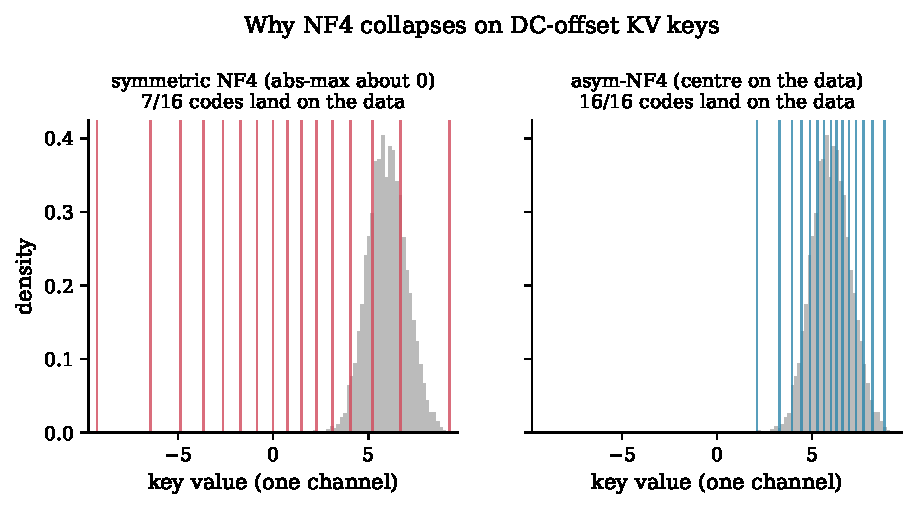
\includegraphics[width=\linewidth]{fig_asymnf4.pdf}
\caption{On a DC-offset key channel, symmetric NF4 (left) places most of its 16 codes where
there is no data; asym-NF4 (right) centres the grid, so every code is used.}
\label{fig:asymnf4}
\end{figure}

\paragraph{Breadth.}
Across seven further LongBench tasks (single/multi-doc QA, multi-hop, summarization, dialogue),
asym-NF4 rescues Qwen's NF4 collapse on \emph{every} task: the 7-task average rises from
\collapse{5.3} (NF4) to \textbf{37.3} (asym-NF4) against 41.1 (fp16). It is near-fp16 on the QA
tasks; summarization is the one soft spot, where asym-NF4 trails fp16 more but remains ${\sim}3
\times$ above NF4's collapse. (Full per-task breadth in the released results; Llama/Mistral
breadth in progress.)

\section{Recommendations}
Use asym-NF4 by default. In the released library this is \texttt{TurboQuantKVCache.robust()}.
Symmetric NF4 should not be shipped for unknown or high-GQA models; asymmetric uniform is a
safe but lower-quality fallback. Pre- vs.\ post-RoPE quantization is a model-specific
micro-optimization (it helps Llama-2-7B but hurts Llama-2-13B and Mistral) and is not a
recommended default.

\section{Limitations}
Four models $\le$13B; LongBench English and WikiText-2; no MoE or $>$13B models. Calibrated
KVQuant/KIVI are compared in-harness on Llama-2-7B only; a broader calibrated comparison is
future work. The GQA-ratio--tolerance hypothesis is tested on four points.

\section{Reproducibility}
All results come from a single harness with JSON-recorded numbers and a notebook offering a
single-GPU subset and a multi-GPU full mode (\texttt{benchmarks/kvquant\_matrix/}).

\end{document}
